\documentclass{beamer}
\usepackage[utf8]{inputenc}
\usepackage[T1]{fontenc}
\usepackage[bulgarian]{babel}
\usepackage{alltt}
\usepackage{graphicx}
\usepackage{amsmath}
\usepackage{yfonts}
\usepackage{amssymb}
\usetheme{Szeged}
\usecolortheme{beaver}

\title[ИС за телекомуникационна компания]{Информационна система за телекомуникационна компания}
\author{\tiny {Емил Станчев, 71100 \\
	Валентина Динкова, 71112 \\
	Ивайло Михайлов, 71102 \\
	Николай Варадинов, 71122 \\
	Мария Григорова, 71058 \\
	Станислав Трифонов, 71094 
	}
	}
\institute{ФМИ}
\date{\tiny{\today}}

\begin{document}

\begin{frame}
  \titlepage
\end{frame}
%\begin{frame}
  %\frametitle{Съдържание}
  %\tableofcontents
%\end{frame}

\section{Потребителски случаи}
\begin{frame}
  \frametitle{Вписване и отписване от системата, регистрация}
    \begin{itemize}
      \item Чрез потребителско име и парола
      \item Поддържа се възстановяване на забравена парола
      \item Достъпно е само през работното време на компанията
      \item Нови потребители се регистрират само от администратор
    \end{itemize}
\end{frame}

\begin{frame}
  \frametitle{Добавяне на нов договор}
    \begin{itemize}
	\item Дата и срок на договора
	\item За дадени устройства и обекти на клиента
	\item Подходящ за принтиране формат
    \end{itemize}
\end{frame}

\section{Домейн модел}
\begin{frame}
  \frametitle{Домейн модел}
  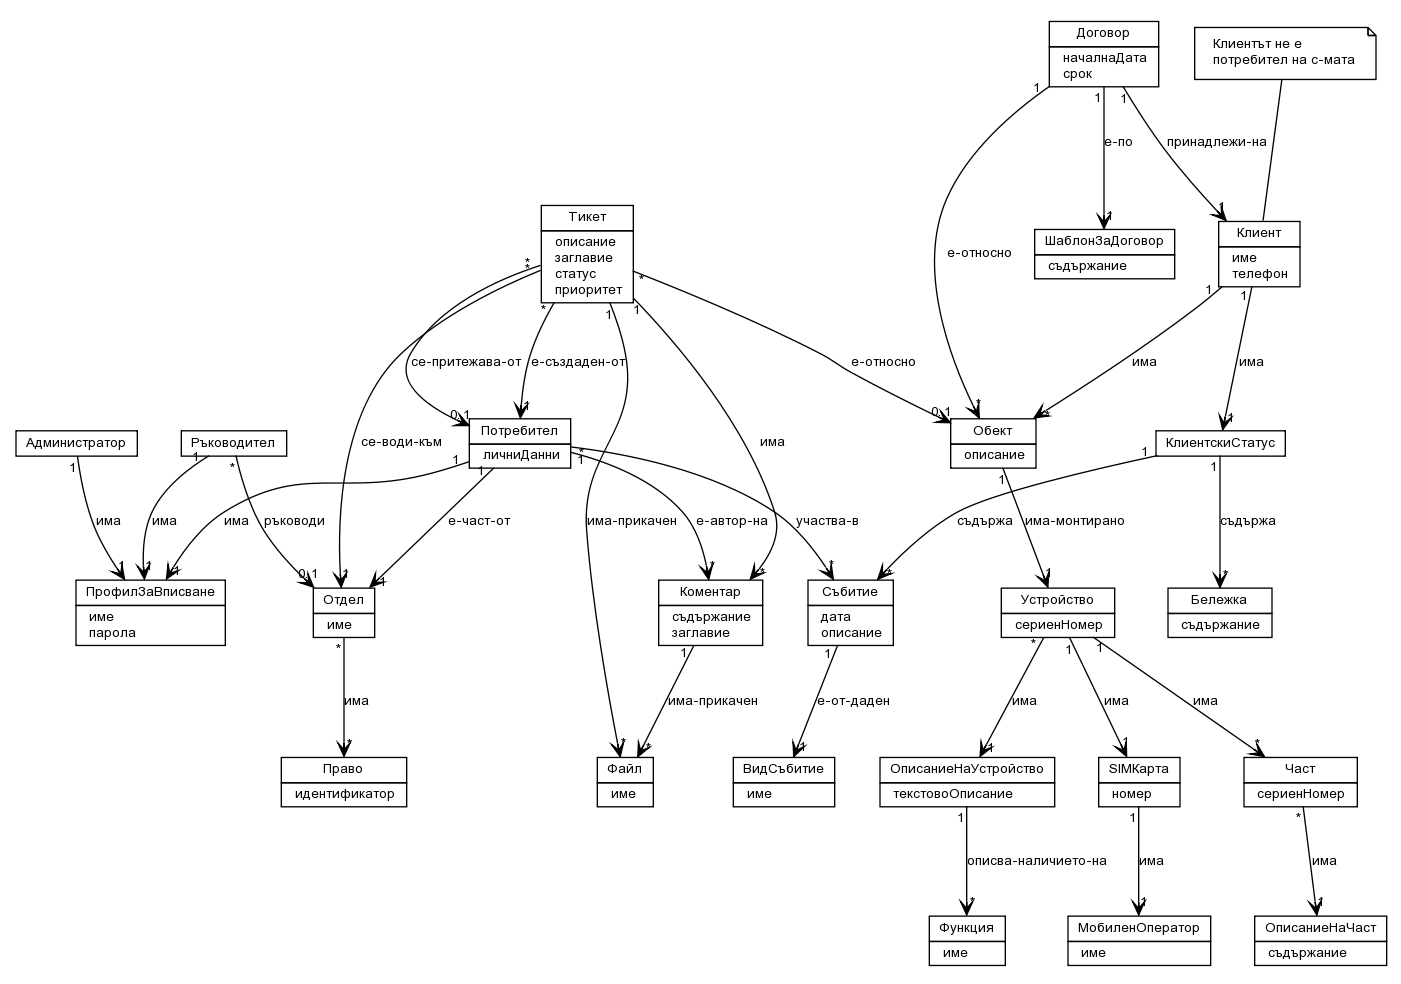
\includegraphics[width= 0.7\paperwidth]{../diagrams/domain.png}
\end{frame}

\end{document}
